\everymath{\displaystyle}
\documentclass{beamer}
% \documentclass[handout]{beamer}

%\usepackage[pdftex]{color,graphicx}
\usepackage{amsmath,amssymb,amsfonts}

\mode<presentation>
{
  % \usetheme{Darmstadt}
  % \usetheme[hideothersubsections]{Hannover}
  % \usetheme[hideothersubsections]{Goettingen}
  \usetheme[hideothersubsections, right]{Berkeley}

  \usecolortheme{seahorse}
  % \usecolortheme{dolphin}
  \usecolortheme{rose}
  % \usecolortheme{orchid}

  \useinnertheme[shadow]{rounded}

  % \setbeamercovered{transparent}
  \setbeamercovered{invisible}
  % or whatever (possibly just delete it)
}

\mode<handout>{
  \setbeamercolor{background canvas}{bg=black!5}
  \usepackage{pgfpages}
  \pgfpagesuselayout{4 on 1}[a4paper,border shrink=5mm, landscape]
}

\usepackage[brazilian]{babel}
% or whatever

% \usepackage[latin1]{inputenc}
\usepackage[utf8]{inputenc}
% or whatever

\usepackage{times}
%\usepackage[T1]{fontenc}
% Or whatever. Note that the encoding and the font should match. If T1
% does not look nice, try deleting the line with the fontenc.


\title%[] % (optional, use only with long paper titles)
{Métodos não paramétricos}

\subtitle
{Ou: o que fazer caso seus dados não sejam normais?} % (optional)

\author%[] % (optional, use only with lots of authors)
{Felipe Figueiredo}% \and S.~Another\inst{2}}
% - Use the \inst{?} command only if the authors have different
%   affiliation.

\institute[INTO] % (optional, but mostly needed)
{Instituto Nacional de Traumatologia e Ortopedia
}
  % \inst{1}%
  % Department of Computer Science\\
  % University of Somewhere
  % \and
  % \inst{2}%
  % Department of Theoretical Philosophy\\
  % University of Elsewhere}
% - Use the \inst command only if there are several affiliations.
% - Keep it simple, no one is interested in your street address.

\date%[] % (optional)
{}

% \subject{Talks}
% This is only inserted into the PDF information catalog. Can be left
% out. 



% If you have a file called "university-logo-filename.xxx", where xxx
% is a graphic format that can be processed by latex or pdflatex,
% resp., then you can add a logo as follows:

\pgfdeclareimage[height=1.6cm]{university-logo}{../logo}
\logo{\pgfuseimage{university-logo}}



% Delete this, if you do not want the table of contents to pop up at
% the beginning of each subsection:
\AtBeginSubsection[]
%\AtBeginSection[]
{
  \begin{frame}<beamer>{Sumário}
    \tableofcontents[currentsection,currentsubsection]
  \end{frame}
}


% If you wish to uncover everything in a step-wise fashion, uncomment
% the following command: 

% \beamerdefaultoverlayspecification{<+->}

\usepackage[normalem]{ulem}

\begin{document}

\begin{frame}
  \titlepage
\end{frame}

\begin{frame}{Sumário}
  \tableofcontents
  % You might wish to add the option [pausesections]
\end{frame}


%% Template
% \section{}

% \subsection{}

% \begin{frame}{}
%   \begin{itemize}
%   \item 
%   \end{itemize}
% \end{frame}

% \begin{frame}
%   \begin{columns}
%     \begin{column}{5cm}
%     \end{column}
%     \begin{column}{5cm}
%     \end{column}
%   \end{columns}
% \end{frame}

% \begin{frame}{}
%   \includegraphics[height=0.4\textheight]{file1}
%   \includegraphics[height=0.4\textheight]{file2}
%   \includegraphics[height=0.4\textheight]{file3}
%   \begin{figure}
%     \caption{}
%   \end{figure}
% \end{frame}

% \begin{frame}{}
%   \begin{definition}
%   \end{definition}
%   \begin{example}
%   \end{example}
%   \begin{block}{Exercício}
%   \end{block}
% \end{frame}

\section{Discussão da aula passada}

\subsection{Discussão da aula passada}

\begin{frame}{Discussão da aula passada}
  \begin{block}{}
    Discussão da leitura obrigatória da aula passada
  \end{block}
\end{frame}

\section{Normalidade}

\begin{frame}{A hipótese da normalidade}
  \begin{itemize}
    \small
  \item Todos os métodos que vimos até aqui presumem que os dados são normalmente distribuídos
  \item Desvios da normalidade precisam ser contornados\footnote{há controvérsias: {\tiny  \url{https://www.r-bloggers.com/normality-tests-don't-do-what-you-think-they-do/}}}
    \bigskip
  \item Veremos duas maneiras: transformações e alternativas
  \end{itemize}
    \bigskip
  \begin{block}{Mas antes...}
    ... como identificar essa necessidade?
  \end{block}
\end{frame}

\subsection{Visualização}

\begin{frame}{Visualização - Histograma}
  \centering
  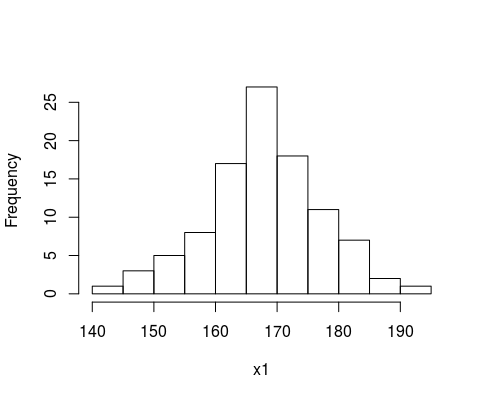
\includegraphics[width=.7\textwidth]{Cap37-38/normal1-h}

  Dados normais
\end{frame}

\begin{frame}{Visualização - Histograma}
  \centering
  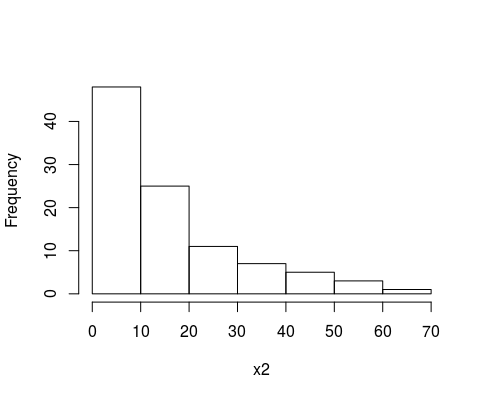
\includegraphics[width=.7\textwidth]{Cap37-38/lognormal1-h}

  Dados não normais
\end{frame}

\begin{frame}{Visualização - Histograma}
  \centering
  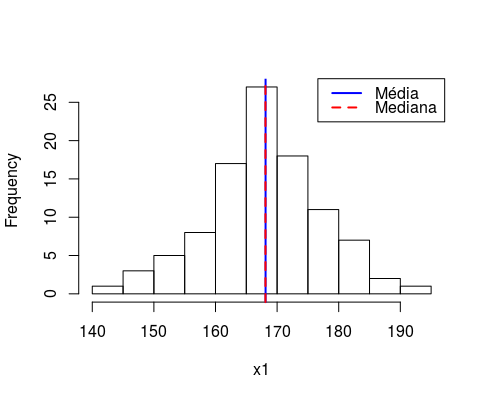
\includegraphics[width=.7\textwidth]{Cap37-38/normal2-h}

  Dados normais
\end{frame}

\begin{frame}{Visualização - Histograma}
  \centering
  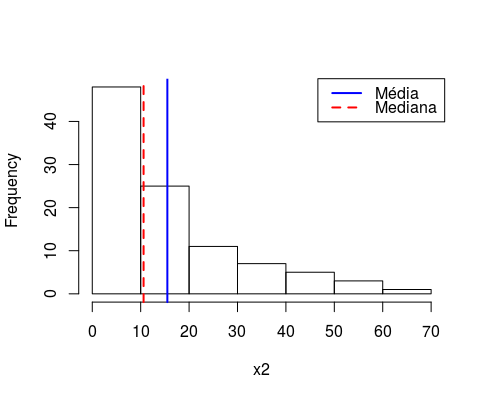
\includegraphics[width=.7\textwidth]{Cap37-38/lognormal2-h}

  Dados não normais
\end{frame}

\begin{frame}{Visualização - Histograma}
  \centering
  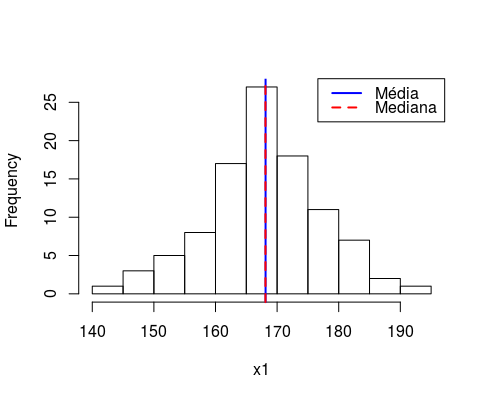
\includegraphics[width=.5\textwidth]{Cap37-38/normal2-h}
  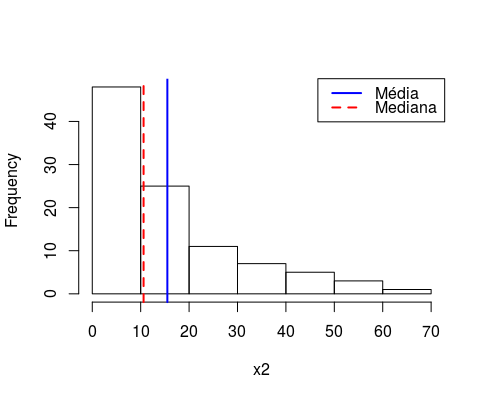
\includegraphics[width=.5\textwidth]{Cap37-38/lognormal2-h}
\end{frame}

\begin{frame}{Visualização - boxplot}
  \centering
  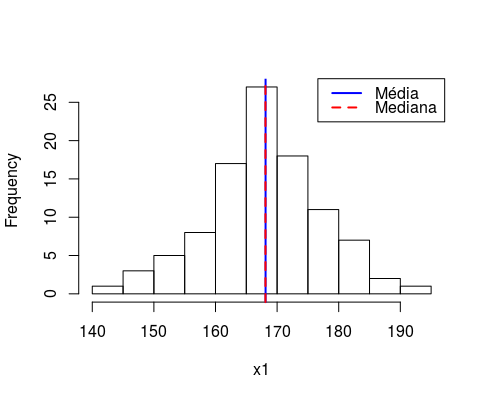
\includegraphics[height=.5\textheight]{Cap37-38/normal2-h}
  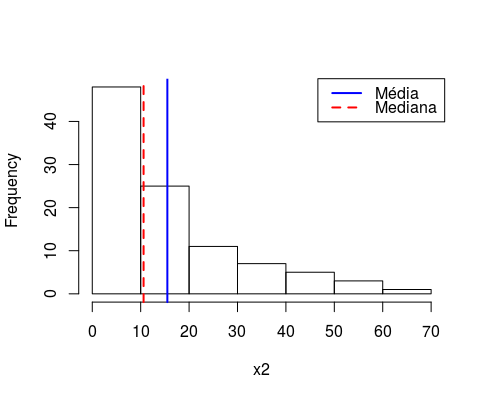
\includegraphics[height=.5\textheight]{Cap37-38/lognormal2-h}

  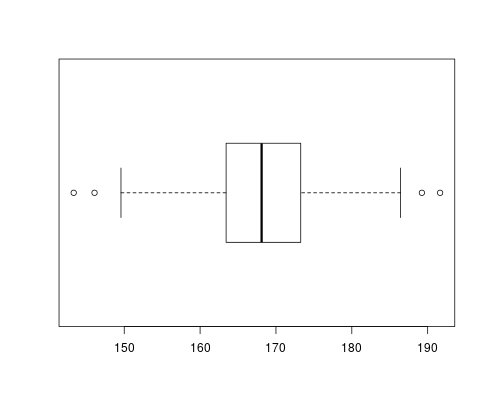
\includegraphics[height=.5\textheight]{Cap37-38/normal-bp}
  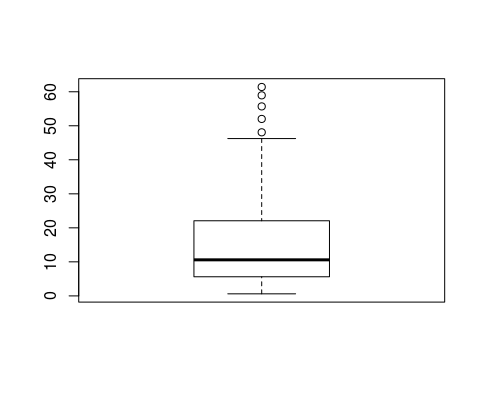
\includegraphics[height=.5\textheight]{Cap37-38/lognormal-bp}
\end{frame}

\begin{frame}{O Q-Q plot}
  \begin{itemize}
    \small
  \item Gráfico que compara os quantis da amostra com os quantis teóricos
  \item Adicionalmente uma reta ``ideal'' é sobreposta, como referência
    \bigskip
  \item Dados normalmente distribuídos ficam próximos da reta
  \end{itemize}
  \bigskip
  \begin{block}{Princípio}
    Quanto maior o desvio da normalidade...

    \bigskip
    ... maior a distância à reta
  \end{block}
\end{frame}

\begin{frame}{Visualização - QQ plot}
  \centering
  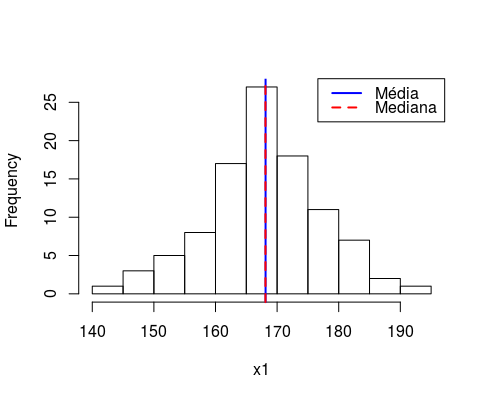
\includegraphics[height=.5\textheight]{Cap37-38/normal2-h}
  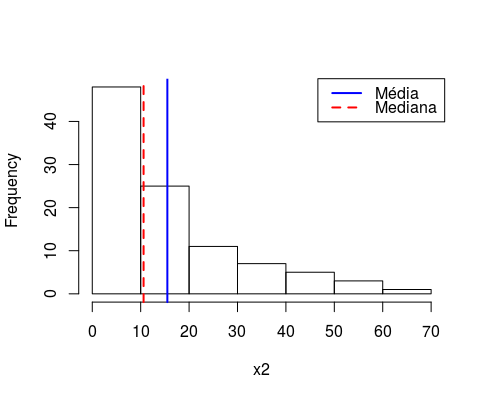
\includegraphics[height=.5\textheight]{Cap37-38/lognormal2-h}

  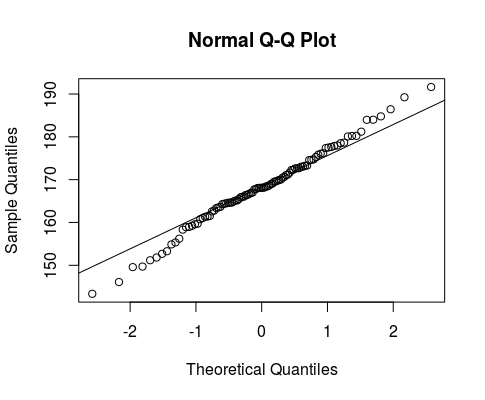
\includegraphics[height=.5\textheight]{Cap37-38/normal-qq}
  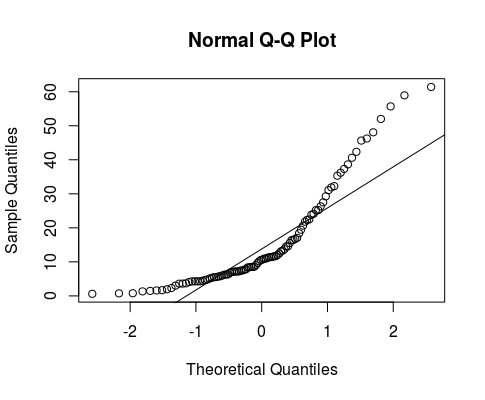
\includegraphics[height=.5\textheight]{Cap37-38/lognormal-qq}
\end{frame}

\subsection[Normalidade]{Testes contra a normalidade}

\begin{frame}
  \begin{itemize}
  \item Objetivo: é possível \alert{determinar} se uma amostra veio de uma população normalmente distribuída?
  \item<2-> Resposta curta: \alert<3->{NÃO}.
    \bigskip
    \bigskip
  \item<4-> Resposta longa: podemos examinar se há evidências para ``aceitar'' esta hipótese\footnote{\scriptsize Lembre: {\bf nunca} aceitamos uma hipótese -- apenas deixamos de rejeitar $H_0$.}
  \end{itemize}
\end{frame}

\begin{frame}{Alguns testes contra a normalidade}
  \begin{itemize}
  \item<1-> \alert<2>{Shapiro-Wilk}
    \bigskip
  \item<1-> Anderson-Darling
    \bigskip
  \item<1-> Kolmogorov-Smirnov
  \end{itemize}
\end{frame}

\begin{frame}{\small Shapiro-Wilk -- Rejeitamos a $H_0$ de normalidade?}
  \centering
  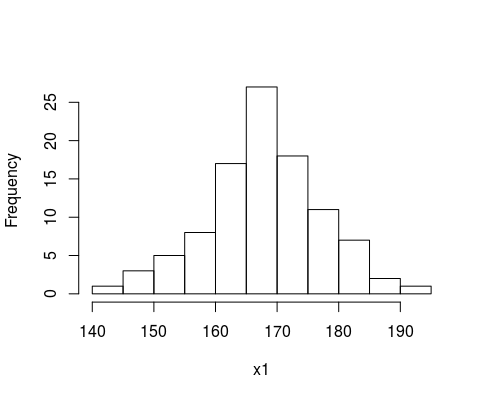
\includegraphics[width=.8\textwidth]{Cap37-38/normal1-h}

  \footnotesize
  \uncover<2>{p-value = 0.7766}
\end{frame}


\begin{frame}{\small Shapiro-Wilk -- Rejeitamos a $H_0$ de normalidade?}
  \centering
  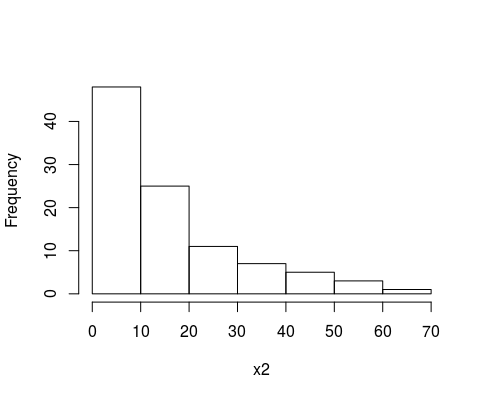
\includegraphics[width=.8\textwidth]{Cap37-38/lognormal1-h}

  \footnotesize
  \uncover<2>{p-value = 1.657e-09}
\end{frame}

\section{Transformações}

\subsection{Transformações}

\begin{frame}{Transformações}
  \begin{itemize}
    \small
  \item Podemos aplicar uma transformação nos dados, para coagi-los a se aproximar das premissas requeridas
    \bigskip
  \item Transformações usuais incluem:
    \begin{itemize}
      \footnotesize
    \item logaritmo
    \item exponencial
    \item raiz quadrada
    \item potências
    \end{itemize}
    \bigskip
  \item Geralmente envolve tentativa e erro \footnote{\scriptsize Mas a transformação de Box-Cox pode ajudar!}
    \bigskip
    \footnotesize
  \item {\bf Hipóteses sobre o problema ou desenho experimental ajudam}
  \end{itemize}
\end{frame}

% \subsection{Exemplo}

\begin{frame}{Exemplo}
  \centering
  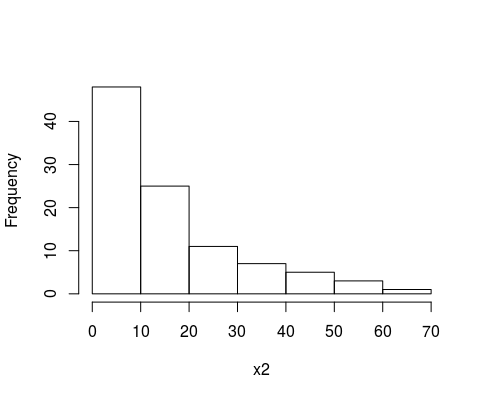
\includegraphics[width=.8\textwidth]{Cap37-38/lognormal1-h}

  \footnotesize
Transformação sugerida: logaritmo.
\end{frame}

\begin{frame}{Exemplo}
  \centering
  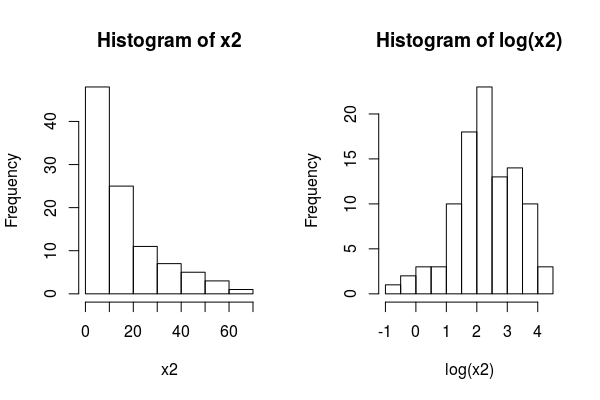
\includegraphics[width=\textwidth]{Cap37-38/transf-h}

  \footnotesize
Dados normais x dados log-transformados
\end{frame}

\begin{frame}{Exemplo}
  \centering
  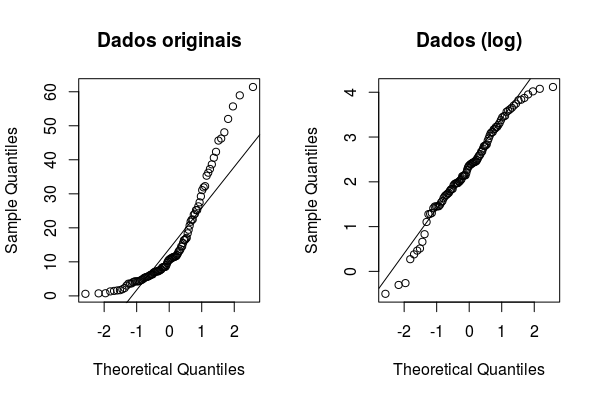
\includegraphics[width=\textwidth]{Cap37-38/transf-qq}

  \footnotesize
(p-valor S-W: 1.657e-09)\ x\ (p-valor S-W: 0.05032)
\end{frame}

\section{Métodos não paramétricos}

\subsection[1 amostra]{Teste para 1 amostra}

\begin{frame}{Teste para 1 amostra}
  \begin{itemize}
  \item Desvios da normalidade severos impactam os testes paramétricos
  \item Nesses casos, deve-se transformar os dados, se possível
  \item Caso não seja, deve-se usar um teste não paramétrico
  \end{itemize}
  \begin{block}{Teste para uma amostra}
    Ao invés do teste t, usar o teste de Wilcoxon (Capítulo 25)
  \end{block}
\end{frame}

\begin{frame}{Quais são as variáveis?}
  \begin{itemize}
    \small
  \item Dependente:
    \begin{itemize}
      \footnotesize
    \item categórica ordinal
    \item numérica discreta
    \item numérica contínua
    \end{itemize}
  \item Independente: parâmetro fixo
  \end{itemize}
  \vfill
  \begin{block}{Esta relação pode ser expressa como}
    \begin{displaymath}
      \text{escore HHS mediano} \sim \text{70}
    \end{displaymath}
  \end{block}
\end{frame}

\subsection[2 médias]{Testes para 2 amostras}

\begin{frame}{Testes para 2 amostras}
  \begin{block}{Dados normais}
    \begin{itemize}
    \item amostras independentes $\Rightarrow$ t-teste não pareado
    \item amostras pareadas $\Rightarrow$ t-teste pareado
    \end{itemize}
  \end{block}
  \begin{block}{Dados não normais}
    \begin{itemize}
    \item amostras independentes $\Rightarrow$ \alert{Mann-Whitney} (Capítulo 24)%\footnote{Também conhecido como Wilcoxon (rank sum test)}
    \item amostras pareadas $\Rightarrow$ Wilcoxon (Capítulo 25)
    \end{itemize}
  \end{block}
\end{frame}

\begin{frame}{Quais são as variáveis?}
  \begin{itemize}
    \small
  \item Dependente:
    \begin{itemize}
      \footnotesize
    \item categórica ordinal
    \item numérica discreta
    \item numérica contínua
    \end{itemize}
  \item Independente:
    \begin{itemize}
      \footnotesize
    \item categórica ordinal
    \item numérica discreta
    \item numérica contínua
    \end{itemize}
  \end{itemize}
  \vfill
  \begin{block}{Esta relação pode ser expressa como}
    \begin{displaymath}
      \text{escore HHS} \sim \text{escore ASA}
    \end{displaymath}
  \end{block}
\end{frame}

\begin{frame}{Em termos práticos...}
P: Estas amostras são significativamente diferentes?

  \centering
  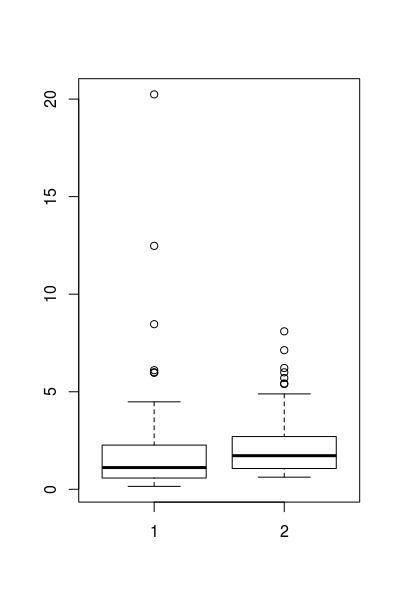
\includegraphics[height=\textheight]{Cap37-38/2samples-bp}
\end{frame}

\begin{frame}{Exemplo}
  \begin{itemize}
  \item<1-> Assumindo\footnote{pelo desenho experimental} que elas são
    \begin{itemize}
    \item<1-> \alert<3>{normalmente distribuídas}, e
    \item<1-> independentes,
    \end{itemize}
poderíamos fazer um teste t não pareado.

  \item<2-> Resultado: p-valor = \alert{0.259}
  \begin{exampleblock}{Pergunta}
    Isto significa que as amostras não são significativamente diferentes?
  \end{exampleblock}
  \end{itemize}
\end{frame}

\begin{frame}{Novamente...}
  \centering
  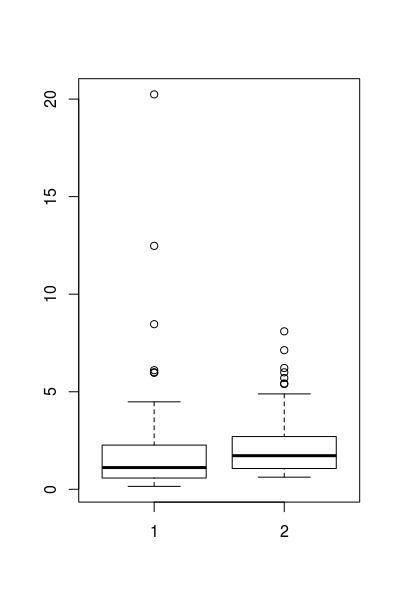
\includegraphics[height=\textheight]{Cap37-38/2samples-bp}
\end{frame}

\begin{frame}{Histogramas}
  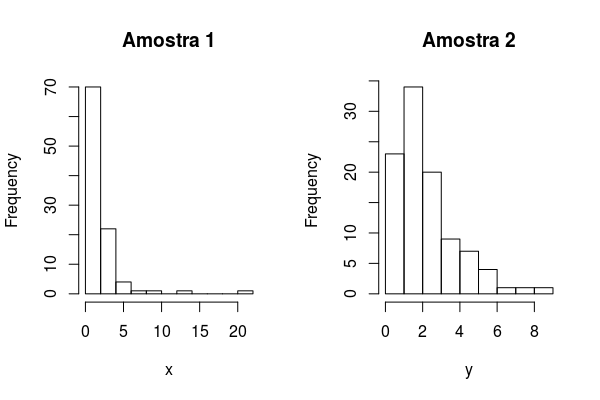
\includegraphics[width=\textwidth]{Cap37-38/2samples-h}

%p-valores Shapiro-Wilk: (x) =  5.515e-16, (y) = 5.274e-09
\end{frame}

\begin{frame}{QQ-plots}
 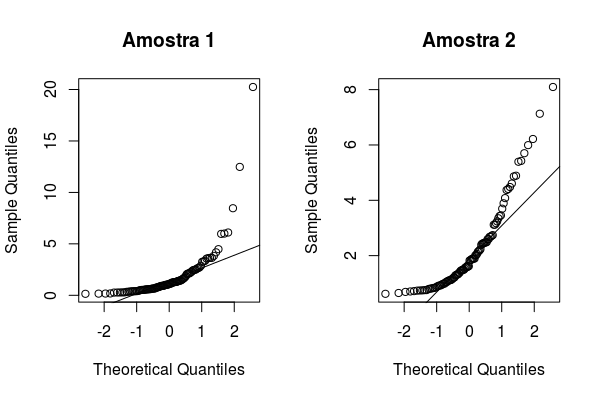
\includegraphics[width=\textwidth]{Cap37-38/2samples-qq}

%p-valores Shapiro-Wilk: (x) =  5.515e-16, (y) = 5.274e-09
\end{frame}

\begin{frame}{Mann-Whitney}
  \begin{exampleblock}{Teste t}
    p-valor = 0.259 (não significativo)
  \end{exampleblock}
  \begin{itemize}
  \item<2-> Aplicando o teste de Shapiro-Wilk em x e y
    \begin{itemize}
    \item<2-> x: p-valor = 5.515e-16
    \item<2-> y: p-valor = 5.274e-09
    \end{itemize}
  \item Devemos rejeitar a hipótese de normalidade.
  \item Então o teste t \alert{não é} apropriado!
  \item Substituto: teste de Mann-Whitney
  \end{itemize}
  \begin{exampleblock}{Teste de Mann-Whitney}
    p-value = \alert{0.0001346} (significativo)
  \end{exampleblock}
\end{frame}

\subsection[3+ amostras]{Teste para 3 ou mais amostras}

\begin{frame}{Relembrando}
  \begin{itemize}
  \item Para testar se há diferença significativa em 3 ou mais amostras
    \begin{itemize}
    \item Análise de Variâncias (ANOVA)
    \item Leva em conta as variâncias entre os grupos (\alert{inter})
    \item Leva em conta a variância em cada grupo (\alert{intra})
    \item $H_0:$ Todos os grupos são $=$
    \item $H_1:$ pelo menos um grupo é significativamente $\ne$
    \end{itemize}
  \end{itemize}
\end{frame}

\begin{frame}{Em termos práticos...}
P: Estas amostras são significativamente diferentes?

  \centering
  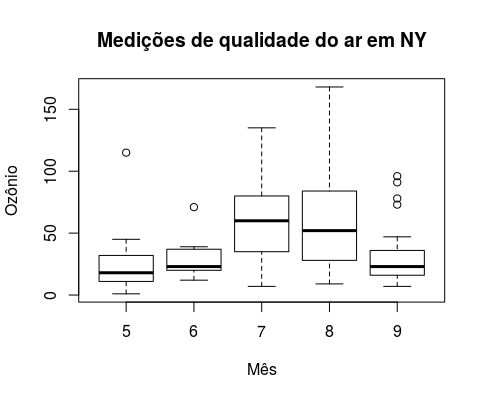
\includegraphics[height=.9\textheight]{Cap37-38/3samples-bp}
\end{frame}

\begin{frame}{Quais são as variáveis?}
  \begin{itemize}
    \small
  \item Dependente:
    \begin{itemize}
      \footnotesize
    \item categórica ordinal
    \item numérica discreta
    \item numérica contínua
    \end{itemize}
  \item Independente:
    \begin{itemize}
      \footnotesize
    \item grupo (categórica nominal -- 3+ níveis)
    \end{itemize}
  \end{itemize}
  \vfill
  \begin{block}{Esta relação pode ser expressa como}
    \begin{displaymath}
      \text{Ozônio} \sim \text{Mês}
    \end{displaymath}
  \end{block}
\end{frame}

\begin{frame}{Kruskal-Wallis}
  \begin{exampleblock}{ANOVA}
    p-valor = 0.0776 (não significativo)
  \end{exampleblock}
  \begin{itemize}
  \item Shapiro-Wilk (Ozônio por mês): $< 0.0001,\ 0.0628,\ 0.86689,\ 0.090325,\ < 0.0001$
  \item Devemos rejeitar a hipótese de normalidade.
  \item Então o ANOVA \alert{não é} apropriado!
  \item Substituto: teste de Kruskal-Wallis (Capítulo 30)
  \end{itemize}
  \begin{exampleblock}{Teste de Kruskal-Wallis}
    p-value = \alert{6.901e-06} (significativo)
  \end{exampleblock}
\end{frame}

\begin{frame}{Pós-teste de Wilcoxon}
  \begin{exampleblock}{Mês x Mês {\small (correção de Bonferroni)}}
    \begin{columns}
      \begin{column}{3cm}
        \begin{itemize}
          \scriptsize
        \item 5 x 6: p = 1.0000
        \item 5 x 7: p = 0.0003
        \item 5 x 8: p = 0.0012
        \item 5 x 9: p = 1.0000
        \item 6 x 7: p = 0.1414
        \item 6 x 8: p = 0.2591
        \item 6 x 9: p = 1.0000
        \item 7 x 8: p = 1.0000
        \item 7 x 9: p = 0.0074
        \item 8 x 9: p = 0.0325
        \end{itemize}
      \end{column}
      \begin{column}{8cm}
        \begin{center}
          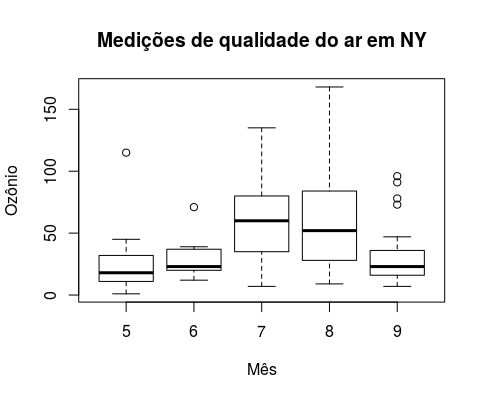
\includegraphics[width=.9\textwidth]{Cap37-38/3samples-bp}
        \end{center}
      \end{column}
    \end{columns}
  \end{exampleblock}
\end{frame}

\subsection{Correlação}

\begin{frame}{Relembrando}
  \begin{itemize}
  \item A correlação de Pearson associa dados numéricos (contínuos)
  \item Mede a direção e força desta associação
  \end{itemize}
  \begin{block}{Correlação não paramétrica}
    Ao invés da correlação linear de Pearson, usar a correlação de ranks de Spearman (Capítulo 17).
  \end{block}
\end{frame}

\section{Resumo}

\begin{frame}{Número de resultados no PUBMED\footnote{Levantamento feito em 2017-11-30}}
  \begin{itemize}
  \item t-test: 61488
  \item ANOVA: 431252
  \item Wilcoxon: 19881
  \item Mann-Whitney: 25571
  \item Kruskal-Wallis: 11943
  \item Shapiro-Wilk: 519
  \item Kolmongorov-Smirnoff: 0
  \item Anderson-Darling: 49
  \item Chi-Square: 107277
  \item OR: 221034
  \item RR: 344996
  \end{itemize}
\end{frame}

\begin{frame}{Resumo (teste oftálmico)}
  % \begin{block}{}
  %     \begin{tabular}{||l||l||}
  %   \hline
  %   Paramétrico & não paramétrico\\
  %   \hline
  %   \hline
  %   t-teste pareado & Wilcoxon\\
  %   \hline
  %   t-teste não pareado & Mann-Whitney\\
  %   \hline
  %   ANOVA 1 fator & Kruskal-Wallis\\
  %   \hline
  %   Correlação de Pearson & Correlação de Spearman\\
  %   \hline
  % \end{tabular}
  % \end{block}
  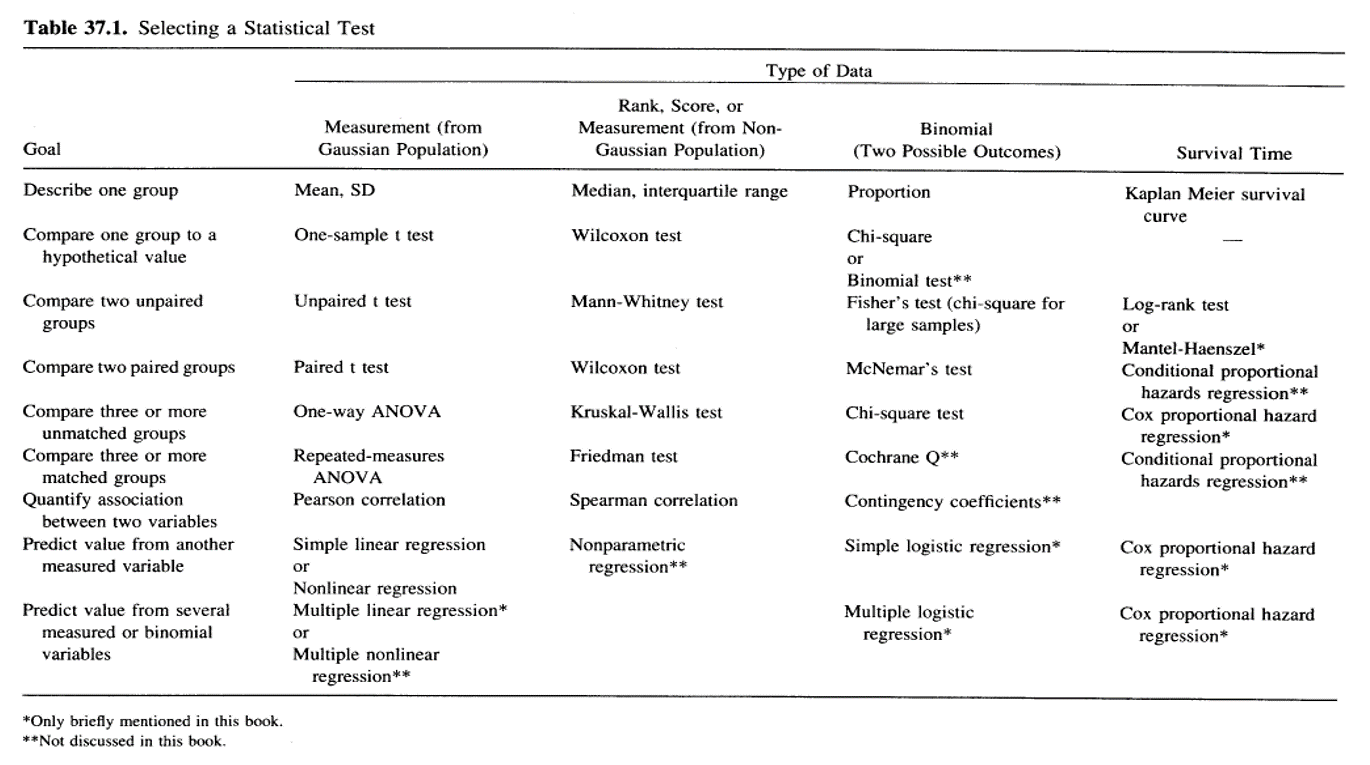
\includegraphics[width=1.2\textwidth]{Cap37-38/metodos1}
\end{frame}

\begin{frame}{Resumo (agora sim)}
  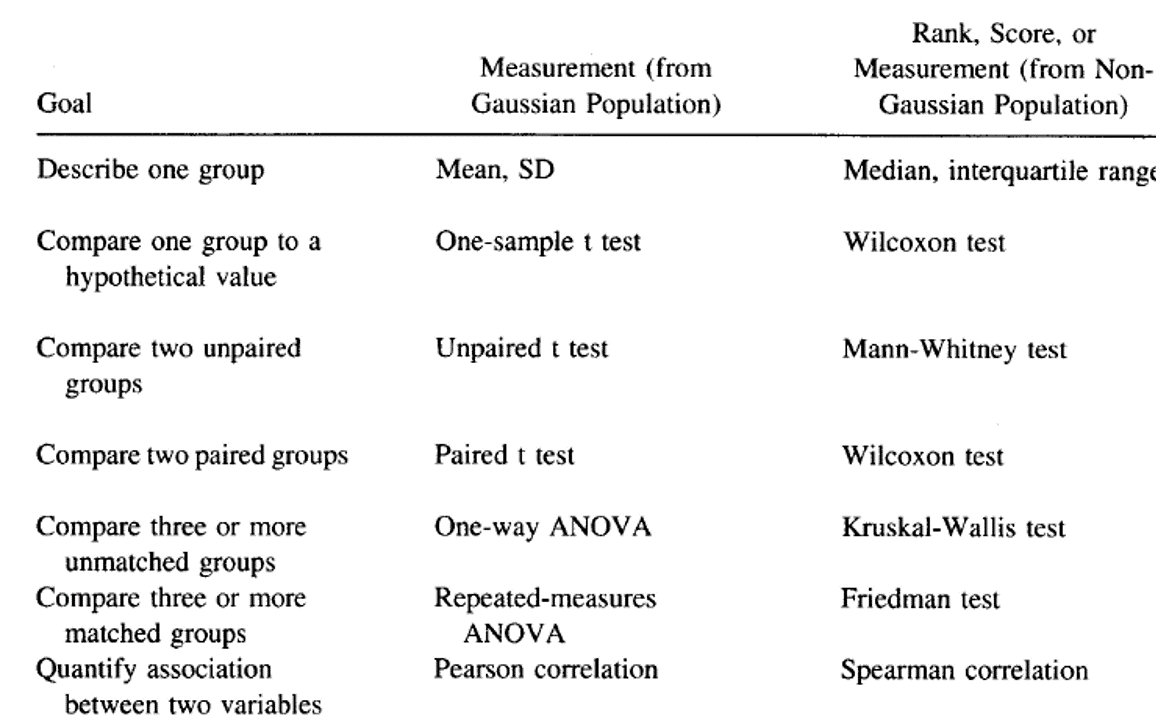
\includegraphics[width=\textwidth]{Cap37-38/metodos2}
\end{frame}

\section{Aprofundamento}

\subsection{Aprofundamento}

\begin{frame}{Aprofundamento}
  \begin{block}{Leitura obrigatória}
    \begin{itemize}
      \small
    \item Capítulo 37
    \item Capítulo 38
    \end{itemize}
  \end{block}
  \begin{block}{Exercícios selecionados}
    \small
    Não há.
  \end{block}
  \begin{block}{Leitura recomendada}
    \begin{itemize}
    \item {\bf Parte VI -- Designing Clinical Trials}
    \scriptsize
    \item Trechos de testes não paramétricos que pulamos dos caps:
      \begin{itemize}
        \scriptsize
      \item 17
      \item 24
      \item 25
      \item 30
      \end{itemize}
    \end{itemize}
  \end{block}
\end{frame}

\end{document}
